\begin{mybilan}
	\begin{itemize}
		\item C'est le mouvement de l'\kw{eau} ou du \kw{vent} qui fournit de l'énergie mécanique à la \kw{turbine d'une centrale hydraulique} ou aux pales d'une \kw{éolienne}. L'eau et le vent sont des \kw{sources d'énergies renouvelables}.
		\item L'alternateur relié à la turbine ou aux pales est l'élément commun aux deux centrales électriques, il transforme l'\kw{énergie mécanique} qu'il reçoit en \kw{énergie électrique} fournie au réseau électrique.
		\item Une partie de l'énergie mécanique est <<\kw{perdue}>> car elle n'est pas convertie en énergie électrique.
		\item On peut traduire la conversion d'énergie par un diagramme d'énergie.
	\end{itemize}

	\begin{center}
		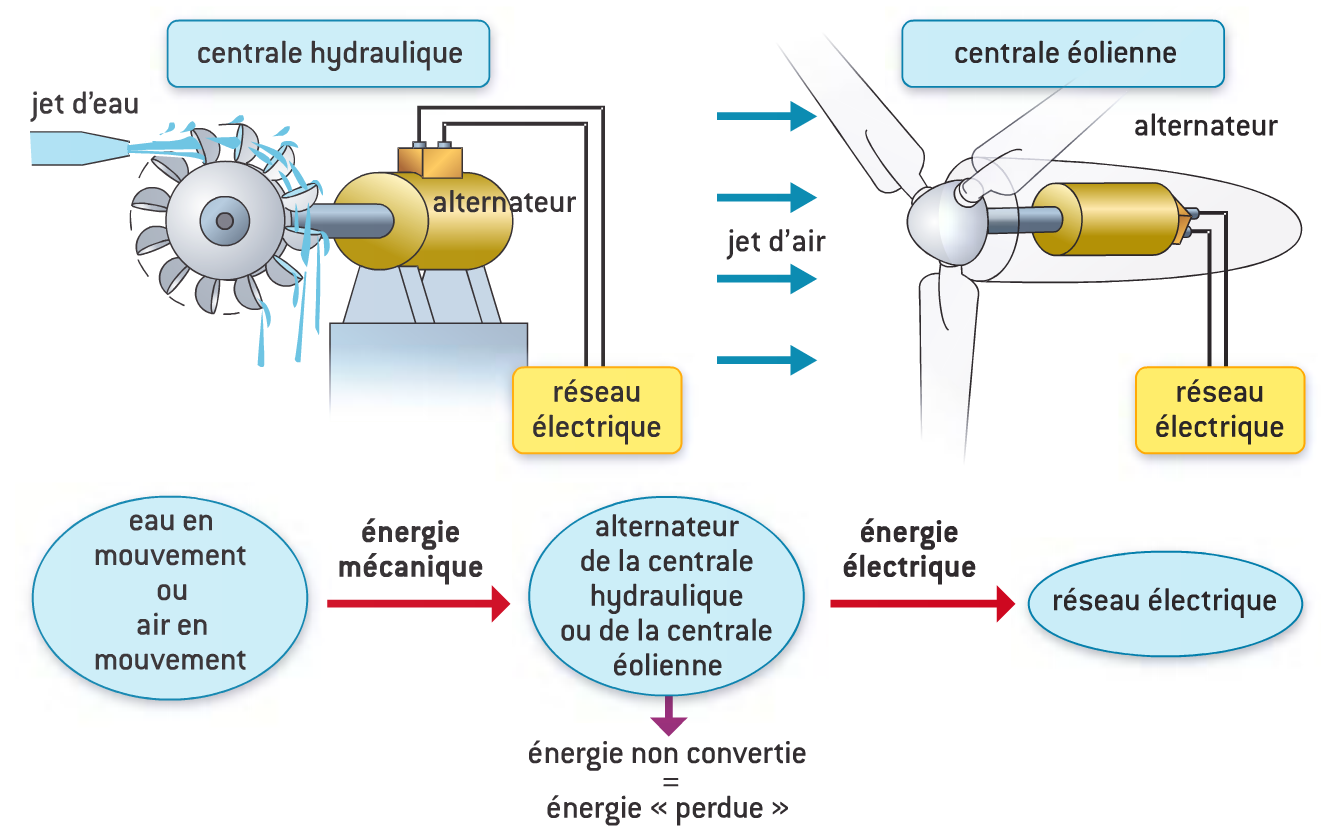
\includegraphics[scale=0.4]{centrales_renouvelables}
	\end{center}
\end{mybilan}